% !TEX root=../thesis.tex

\chapter{Implementation} % (fold)
\label{cha:implementation}
In this chapter we will describe the technology used when developing the 
prototype, and how the technology was implemented. 

\section{Back-end} % (fold)
\label{sec:back_end}
In this section we will describe how the back-end of the system was 
implemented. The back-end is the part of the system which functions as the
interface between the user input from the front-end and data storages, and
mediates data between these.

\subsection{Data storage} % (fold)
\label{sub:back_end_data_storage}
Since the data was given in different sets and some sets serve a different
purposes, different sets was stored differently. For the prototype developed, 
the data was stored in 3 databases although optimally the amount of databases 
would have been two. The increased amount of databases is due to one of the data sets which was given as a interface to an existing database, while the others were given as sets which had to be put into a database.

The first database (The "station database") that was set up, was the one that 
contained the stations.
The structure was determined by the hierarchy of stakeholders presented in
\Ref{sec:back_stakeholders}.  We were presented with a list of all the
relevant stakeholders, which were all the area directors, stretch directors,
and segment director. The hierarchy in the "station database" database ended 
up as presented in the following list and the structure is similar for all 6 
areas and all the different numbers of stretches and segments beneath each 
area.

\begin{itemize}
	\item Area 1
	\begin{itemize}
		\item Strech 1
		\begin{itemize}
			\item Segment 1
		\end{itemize}
		\item Stretch 2
		\begin{itemize}
			\item Segment 2
			\item Segment 3
		\end{itemize}
	\end{itemize}
\end{itemize}


The second and third databases (the "information database(s)") were all built
around the stations. By having the databases built around the stations, the 
relation between these events and the stakeholders were a connection between 
the events and either one or two stations. Since all events had a connection 
to a station, these "information database(s)" all had a similar structure with 
data points such as stations where event occurred, scheduled and actual time 
of arrival and departure and train number. An example of such a data set is 
presented in \Ref{fig:jernbaneverket-trafikkdata}.

% subsection data_storage (end)

\subsection{Aggregation} % (fold)
\label{sub:back_end_aggregation}
When the system shall aggregate for the stakeholders, the front-end sends
the stakeholder, information type, and time parameters to the back end. 
The system then locates the correct stakeholder in the "station database",
which returns the correct area to which the stakeholder belongs. Based on the 
area returned by the database, the information selected, and the time window
selected, the system will fetch the relevant data from the "information 
databases". \\

Since most of the of the information is count based, the aggregation performed
on these sets are a simple average function along with generating dummy 
markers for each sub-area. Say one was to select a area as the current 
stakeholder with crossings as current data type, the system will then loop 
through and average all crossings per station within every segments and 
generate a marker located on the average location of all the stations with the 
average crossing of all these stations. The system will then do the same for 
all segments within one stretch. By performing the aggregation method for a 
area, you end up with a average marker for each stretch, located on the  
average location of all segments generated from all the stations, with the 
average crossings of all stations in that area.\\

The database structure presented above is implemented similar on the other 
sets of data, except in the case of Speed restrictions. The difference in the
datasets is due to that the workshops determined that the speed restrictions
was to be displayed with a own marker limited by the time selector.
% subsection back_aggregation (end)

% section back_end (end)

\section{Front-end} % (fold)
\label{sec:front_end}
In this section we will describe how the front-end was implemented. The
front-end is the part of the system that interacts with the user.

\subsection{Data set presentations} % (fold)
\label{sub:front_end_data_set_presentation}
When presenting the information to the user, the ability to maintain a tidy
presentation but at the same time present all the necessary information is 
important. Since the system shall present different kind of information, a 
selectable list of the implemented information types was implemented. The 
selectable list, presented in \Ref{fig:implementation_type_selection}, sets a 
internal variable which determines what kind of information shall be fetch 
from the databases and in turn be presented to the user.\\

As was mentioned in \Ref{sec:back_aggregation}, speed restrictions were
meant to be displayed as a own marker per event restricted within the selected
time window. In the database, each speed restriction event is stored with an id
which is equal to an image file with the plot. The data query will return with 
the id of each matched event, and the matching images will then be displayed
within the popup of the marker for each event. An example of a speed 
restriction marker with plot is presented in \Ref{fig:speed_restriction_presentation}.\\


Since the other information types were meant to be displayed in a dashboard, a
simple way of displaying the aggregated data along side each marker was made.
An example of a aggregated dashboard is presented in \Ref{fig:crossings_presentation} with the use of number of aggregated crossings in the Oslo area and East area as an example. When a user selects a new information type and the variable is updated, then sends a new request to the back end which in return presents the front-end with new data to present. The system will then dynamically update the dashboards and the markers.

When the time selection was to be implemented, the input method had been
decided to be implemented as input boxes in one of the corners for from and to 
date and time, as presented in \Ref{fig:time_selection_implemented}. When user 
changes the time interval, the input is validated to be in correct form and 
used in the request for data.\\

%TODO endre formulering på avsnittet her
It were also meant to implement a top 5 lists for each information, this was
however not completed. It was meant to display a list of the worst or best of
the information type within each current stakeholders responsible area. In the
case of crossings, the information would display the five stations with the 
most crossings, as demonstrated in \Ref{fig:top_5_list}. The top 5 list was 
demonstrated with static HTML-list of random stations with a random number.

When a request for information have been sent to the back end, the display will
then plot the information in markers. The system will then fit the map
according to a rectangle automatically calculated from the markers.
% subsection data_storage (end)

\subsection{Aggregation} % (fold)
\label{sub:front_end_aggregation}
Since most of the aggregation was done in the back end, there was not much
needed to be done in the front-end. One of the first things implemented, was 
the selection of stakeholders, see \Ref{fig:stakeholder_selection_list}. The
stakeholder is generated dynamically by sending a request for all the 
stakeholders to the back-end, and aggregate through the response which will 
generate the selectable list of stakeholders. 
% subsection back_aggregation (end)


\begin{figure}[h!tbp]
	\centering
	\begin{subfigure}{0.6\textwidth}
		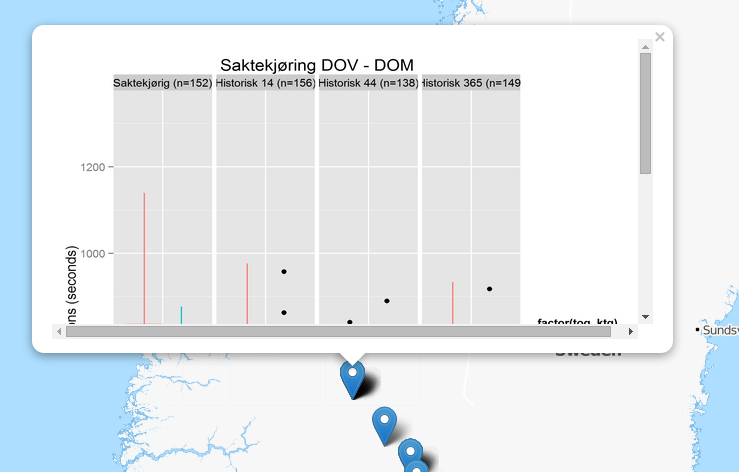
\includegraphics[width=\textwidth]{speed_restriction_presentation.png}
		\caption[Speed restriction presentation]{Speed restriction presentation}
		\label{fig:speed_restriction_presentation}
	\end{subfigure}
	\begin{subfigure}{0.25\textwidth}
		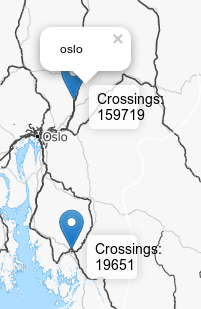
\includegraphics[width=\textwidth]{crossings_presentation.png}
		\caption[Crossings presentation]{Crossings presentation}
		\label{fig:crossings_presentation}
	\end{subfigure}
	\caption[Crossings and Speed restriction implementation]{Crossings and Speed restriction
	implementation}
	\label{fig:crossings_and_speed_restriction_implementation}
\end{figure}

\begin{figure}[h!tbp]
	\centering
	\begin{subfigure}{0.3\textwidth}
		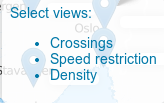
\includegraphics[width=\textwidth]{information_type_selection.png}
		\caption[Implementation type selection]{Implementation type selection}
		\label{fig:implementation_type_selection}
	\end{subfigure}
	\begin{subfigure}{0.6\textwidth}
		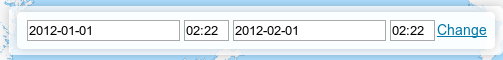
\includegraphics[width=\textwidth]{time_selection_implemented.png}
		\caption[Time selection implementation]{Time selection implementation}
		\label{fig:time_selection_implemented}
	\end{subfigure}
	\caption[Information type and Time selection]{Information type and Time selection}
	\label{fig:information_type_and_time_selection}
\end{figure}

\begin{figure}[h!tbp]
	\centering
	\begin{subfigure}{0.4\textwidth}
		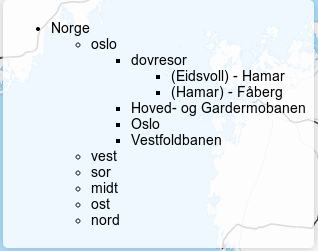
\includegraphics[width=\textwidth]{stakeholder_selection_list.png}
		\caption[Stakeholder selection list]{Stakeholder selection list}
		\label{fig:stakeholder_selection_list}
	\end{subfigure}
	\begin{subfigure}{0.4\textwidth}
		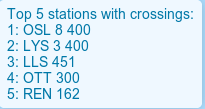
\includegraphics[width=\textwidth]{top5.png}
		\caption[Top 5 list]{Top 5 list}
		\label{fig:top_5_list}
	\end{subfigure}
	\caption[Stakeholder selection and Top 5 list]{Stakeholder selection and Top 5 list}
	\label{fig:stakeholder_selection_and_Top5_list}
\end{figure}

\begin{figure}[!htbp]
	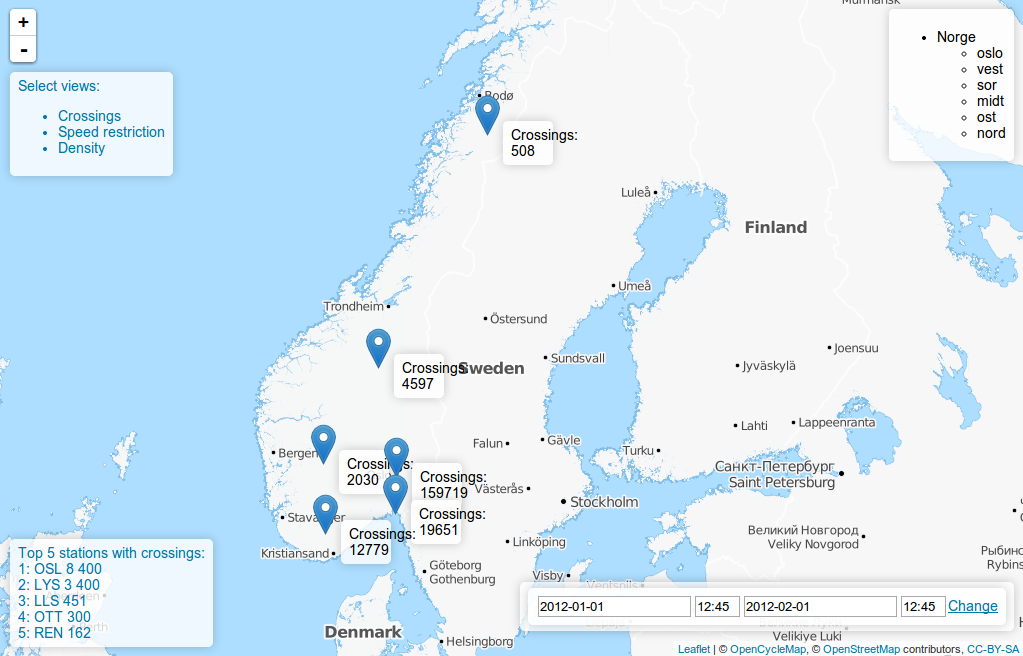
\includegraphics[width=\textwidth,center]{map_prototype.png}
	\caption[Map implementation]{Map implementation}
	\label{fig:map_prototype}
\end{figure}

% section front_end (end)

\section{System architecture} % (fold)
\label{sec:system_architecture}
In this section we will describe the architecture of the implemented prototype.

Keyword:
We used the architectural pattern called "layered pattern"\cite[pp. 205-210]{Bass:2012:SAP:2392670}, which is a three-tier architecture from the database 
point of view\cite[pp. 294-297]{toftHanseMallaugDatabaser}.

\begin{figure}[!htbp]
	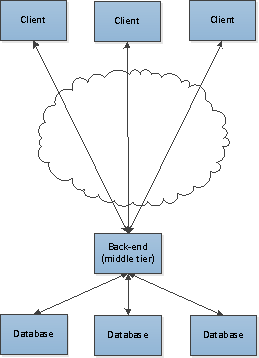
\includegraphics[width=0.5\textwidth,center]{system-communication.png}
	\caption[Three-tier architecture]{Three-tier architecture}
	\label{fig:three-tier_architecture}
\end{figure}
% section system_architecture (end)

\section{Technology} % (fold)
This section will describe the technology used to implement the prototype.
\label{sec:technology}

\subsection{Server} % (fold)
\label{sub:server}
When the back end was due for implementation, Node.js\cite{nodeJs} was chosen 
as the framework for the server. Node.js is a event-driven, non-blocking  I/O
model framework which is based on Chrome's\cite{chromeJavaScriptEngine} 
JavaScript runtime. The Node.js framework enables small, fast, and scalable 
network applications.

When the user wanted to change information type or active stakeholder, the
request for data was posted to the server through a REST\cite{REST} api. An
example of a request for the number of crossings for the Oslo area is
"/rail/numberOfCrossings/2012-01-01/2012-02-01/oslo". The server then uses the
Express\cite{express} framework to parse all get request to the server to send
these request to methods within the Node server which parses these requests.


 % subsection server (end)

\subsection{Data storage} % (fold)
\label{sub:technology_data_storage}
When storing the data, several types of databases was used as mentioned in
\Ref{sub:back_data_storage}. The "station database" was implemented in
a noSQL document database structure called MongoDB\cite{mongoDB}. The MongoDB
database have a structure which on a database holds a set off collections. a
collection holds a set of documents. A documents is a set of key-value pairs.
For this thesis, The MongoDB database structure meant that one can search 
on a single key, for instance the name of an area, and get all relevant data 
within that structure. The MongoDB driver called Monk\cite{npmMonk} was used 
to access the implemented MongoDB database.\\

When setting up the last two databases, more traditional relational databases 
was used. The first database implemented was one in PostgreSQL
\cite{postgreSQLAbout}. The node-postgres\cite{node-postgres} was used to 
access this database. The PostgreSQL database was chosen due the functionality 
of the database and since we were most familiar with PostgreSQL. The 
last database was given as an interface to connect to, and was set up in MySQL
\cite{mySQLAbout}. The node-mysql\cite{node-mysql} driver was used to access 
the given MySQL interface.
% subsection technology_data_storage (end)

\subsection{Map} % (fold)
\label{sub:map}
Since the map was a important part of the presentation of data, the selection
of the map library were an important decision. Leaflet\cite{leaflet} was 
chosen due to the library being a more and more popular library which is open 
source. The Leaflet JavaScript library is designed with simplicity, 
performance and usability in mind.

All functions within the map is an extension of functions that exists in the
map. Information selection, time selection, stakeholder selection and Top 5 is
an extension of the L.Control object. The dashboards uses a standard marker,
and a bit of css to display the marker icon and the information. The map
prototype developed was presented in \Ref{fig:map_prototype}.
% subsection map (end)

% section technology (end)

% chapter implementation (end)
